\begin{center}
    \begin{figure}[H]
        \centering

        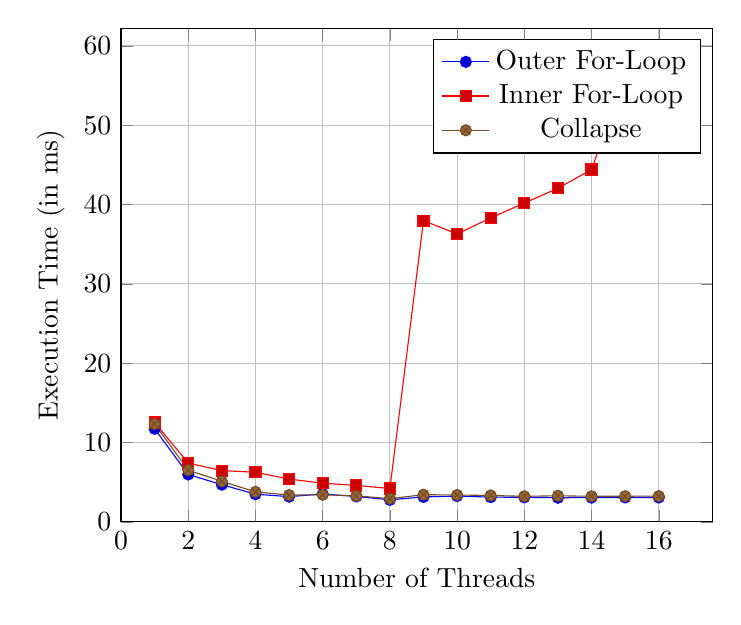
\begin{tikzpicture}
            \begin{axis}[
                title={},
                width=0.75\textwidth,
                xlabel={Number of Threads},
                ylabel={Execution Time (in ms)},
                xmin=0,
                ymin=0,
                grid=major
            ]
                \addplot coordinates {
                    (1,11.7365)(2,5.97965)(3,4.69315)(4,3.49675)(5,3.18585)(6,3.52845)(7,3.20715)(8,2.78265)(9,3.15175)(10,3.2601)(11,3.12815)(12,3.10095)(13,3.05015)(14,3.06365)(15,3.08175)(16,3.07475)
                };
                \addlegendentry{Outer For-Loop}

                \addplot coordinates {
                    (1,12.5315)(2,7.41705)(3,6.46785)(4,6.26345)(5,5.4006)(6,4.88325)(7,4.59995)(8,4.20975)(9,37.9699)(10,36.2843)(11,38.3156)(12,40.1812)(13,42.0504)(14,44.4038)(15,56.4891)(16,55.9547)
                };
                \addlegendentry{Inner For-Loop}       

                \addplot coordinates {
                    (1,12.3462)(2,6.5227)(3,5.1136)(4,3.7885)(5,3.38175)(6,3.42255)(7,3.28445)(8,2.93785)(9,3.43565)(10,3.3931)(11,3.33495)(12,3.2319)(13,3.29275)(14,3.2345)(15,3.2412)(16,3.25085)
                };
                \addlegendentry{Collapse}
            \end{axis}
        \end{tikzpicture}
        \caption{HSV Performance Tests pnglogo-blk.png}
    \end{figure}
\end{center}